\begin{figure}
    \centering
    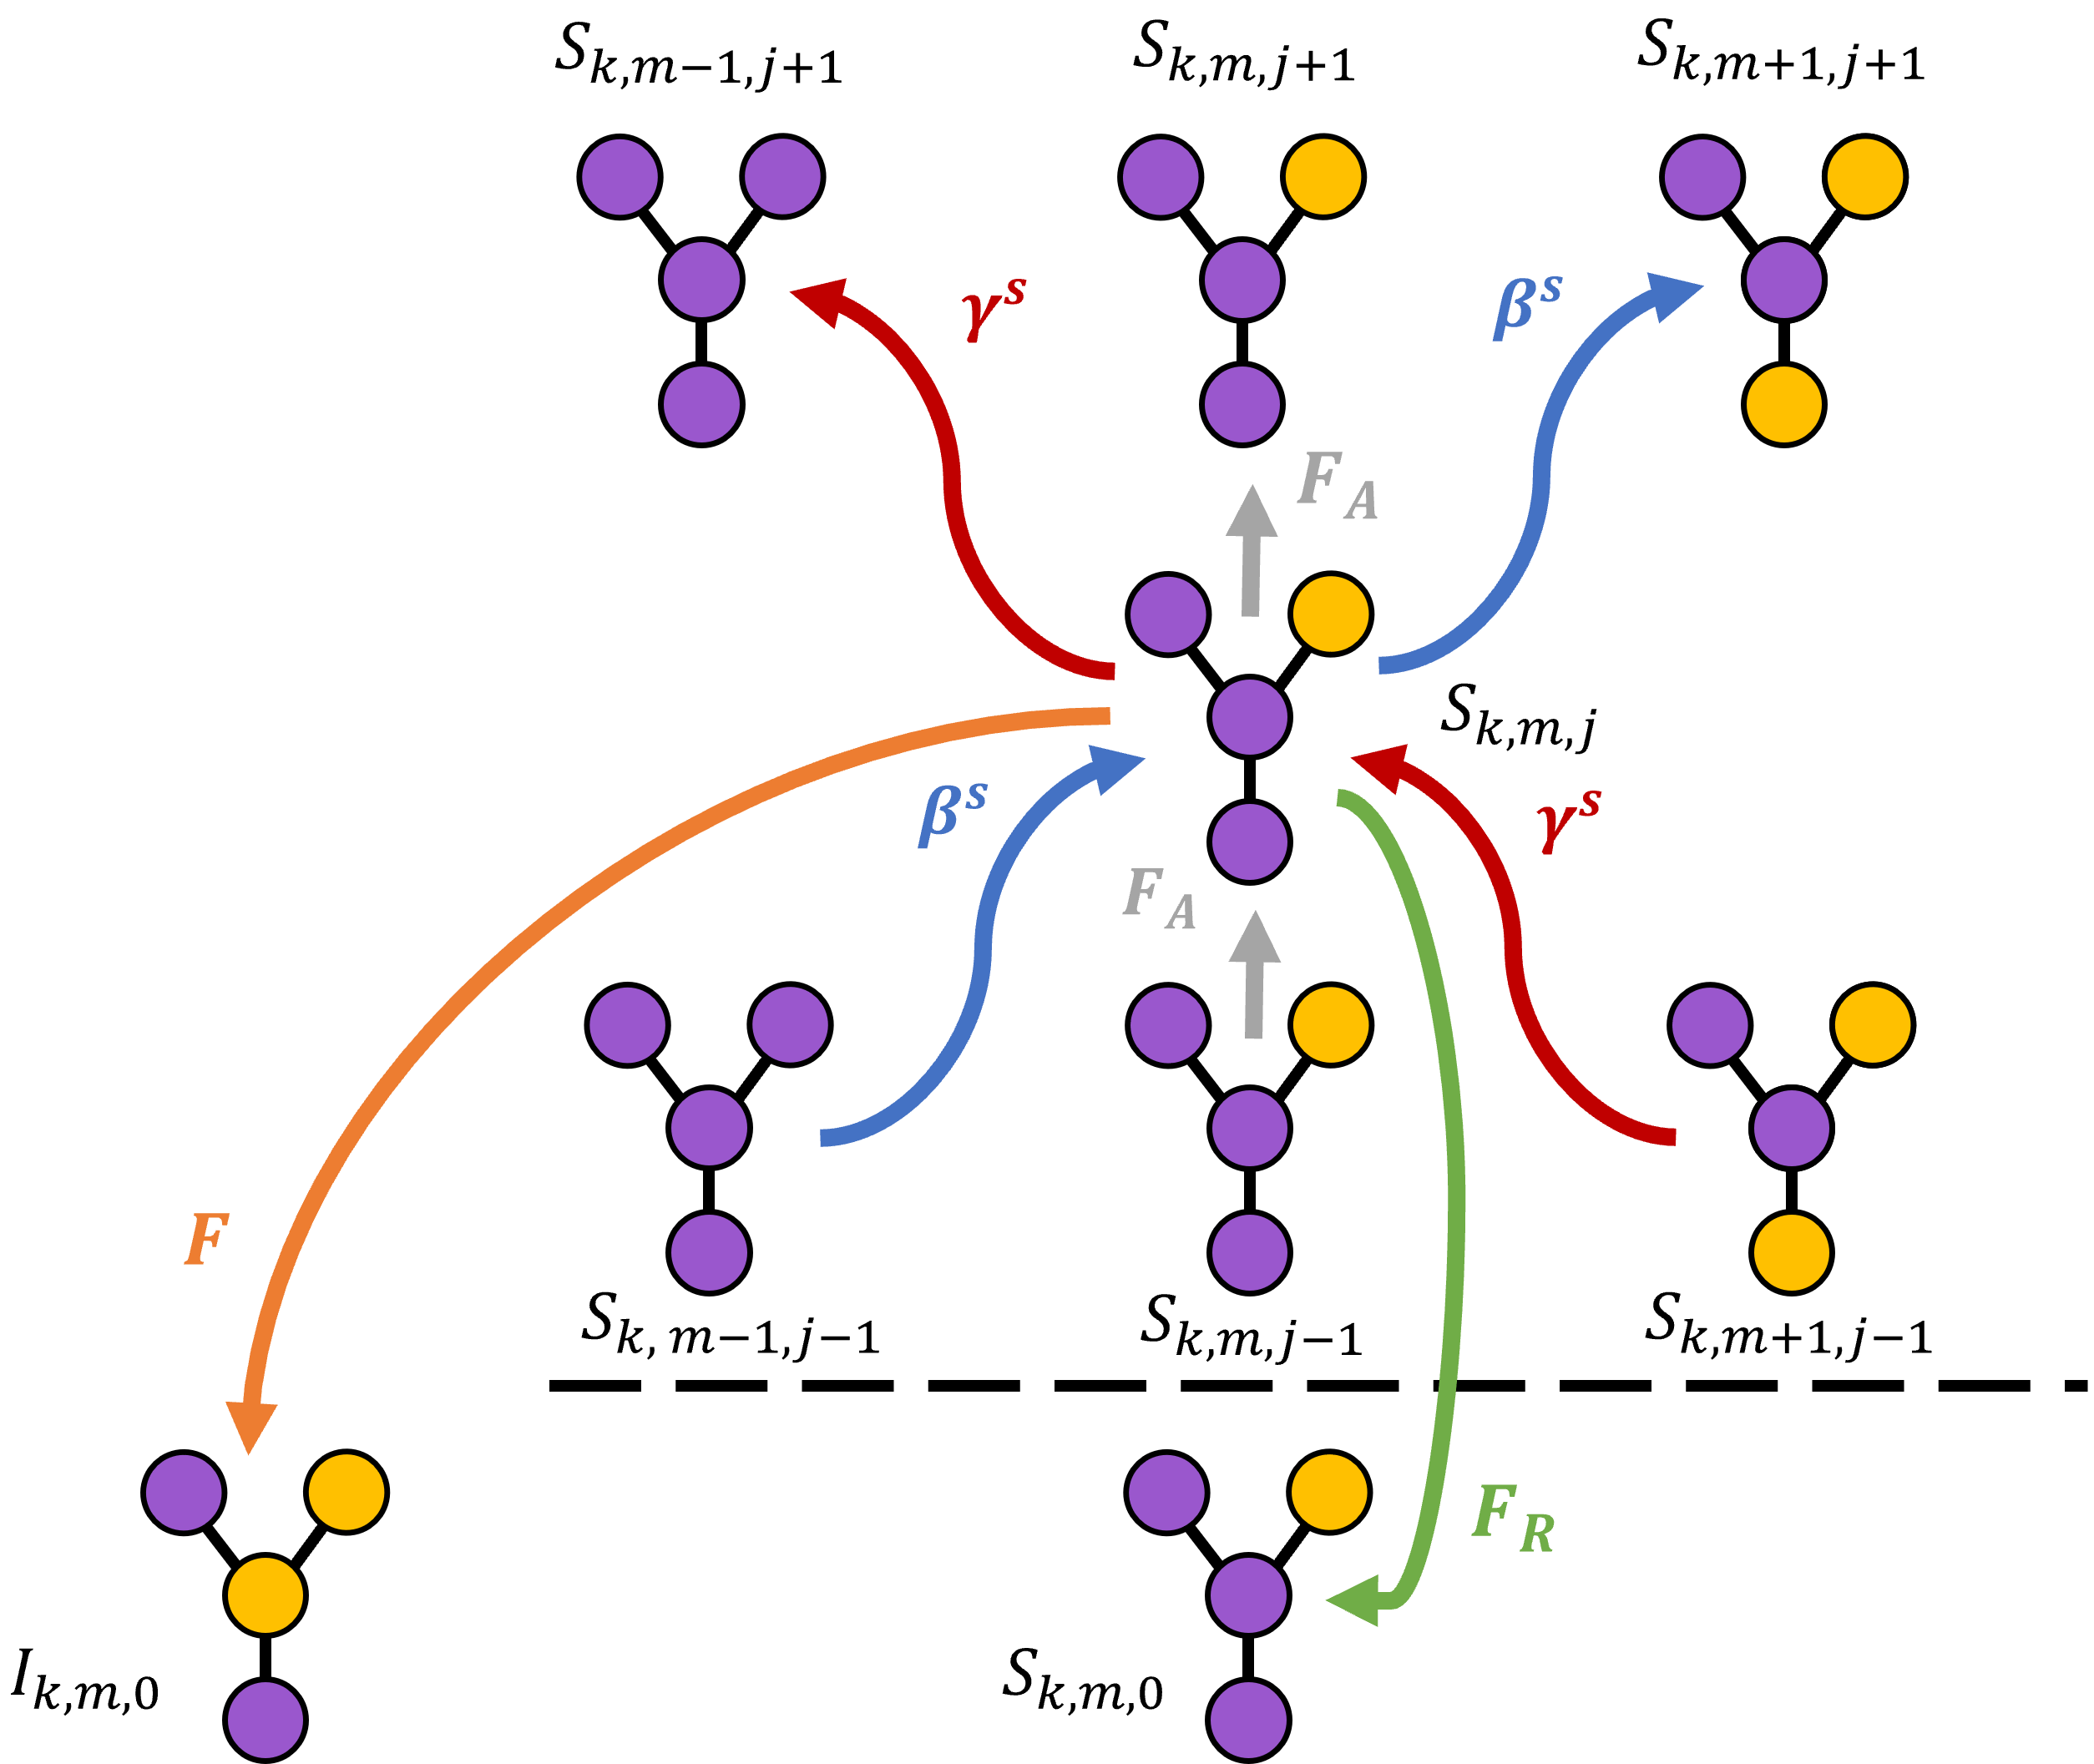
\includegraphics[width=\columnwidth]{Figs/Appendix2_Threshold/AME_PLOT.png}
    \caption[Schematic representation of the transitions to or from the set $s_{k,m,j}$]{\label{fig:ame_plot1} Schematic representation of the transitions to or from the set $s_{k,m,j}$ ($j > 0)$. We show the central node with some neighbors for different values $m$ and $j$. Purple nodes are susceptible or non-adopters or spin-down, and yellow are infected or adopters or spin-up.}
\end{figure}
    
We consider  binary-state dynamics on static, undirected, connected networks assuming a locally tree-like structure and in the limit of $N \to \infty$, following closely the approach used in Ref. \cite{gleeson-2013} for binary-state dynamics in complex networks. The new ingredient  is to consider the nodes with different age as different sets, what allows us to treat as Markovian the memory effects introduced by aging \cite{peralta-2020C,peralta-2020A}. We define $s_{k,m,j} (t)$ ($i_{k,m,j} (t)$) as the fraction of nodes that are susceptible (infected) and have degree $k$, $m$ infected neighbors and age $j$ at time $t$. The networks have degree distribution $p_k$ and have been generated by the configuration model \cite{molloy-1995,newman-2001}. The initial condition is set such that all agents have age $j = 0$ and there is a randomly chosen fraction $\rho_0$ of nodes infected:
\begin{align} \label{initial_condition} 
    \textrm{For } j > 0 & \quad    s_{k,m,j} (0) = 0  \quad   i_{k,m,j} (0) = 0, \nonumber\\
    \\
    \textrm{For } j = 0 & \quad    s_{k,m,0} (0) = (1 -  \rho_0)\, B_{k,m}[\rho_0] \nonumber \\
                        & \quad    i_{k,m,0} (0) = \rho_0\, B_{k,m}[\rho_0], \nonumber
\end{align}
where $B_{k,m}[\rho_0]$ is the binomial distribution with $k$ attempts, $m$ successes and $\rho_0$ is the initial fraction of infected agents that as the probability of success of the binomial. Now, we examine how $s_{k,m,j}$ changes in a time step. We consider separately the case $j = 0$ since its evolution is different from $j > 0$. See Fig. \ref{fig:ame_plot1} for a schematic representation of transitions involving $s_{k,m,j}$.
    
This is the way to reach the expressions of Eq. \eqref{eq:pre_AME}:
\begin{align} \label{eq:pre_AME}
        s_{k,m,j} (t + dt) = & \, s_{k,m,j}(t) - F (k,m,j)\, s_{k,m,j}\, dt - F_{R} (k,m,j)\, s_{k,m,j} \, dt - F_{A} (k,m,j) \, s_{k,m,j} \, dt \nonumber \\
        & + F_{A} (k,m,j-1)\,  s_{k,m,j-1} \, dt - \omega (s_{k,m,j} \to s_{k,m+1,j+1}) \, s_{k,m,j}\, dt  \nonumber \\
        & - \omega (s_{k,m,j} \to s_{k,m-1,j+1})\,  s_{k,m,j} \, dt + \omega (s_{k,m+1,j-1} \to s_{k,m,j}) \, s_{k,m+1,j-1} \, dt \nonumber \\
        & + \omega (s_{k,m-1,j-1} \to s_{k,m-1,j-1}) \, s_{k,m-1,j-1}\,  dt, \\
        s_{k,m,0} (t + dt) = &\,  s_{k,m,0}(t) - F (k,m,0) \, s_{k,m,0} \, dt + \sum_{l = 0}^{\infty} R (k,m,l)\,  i_{k,m,l} \, dt + \sum_{l = 1}^{\infty} F_{R} (k,m,l)\,  s_{k,m,l}\,  dt   \nonumber\\
        & - F_{A} (k,m,0)\,  s_{k,m,0}\,  dt - \omega (s_{k,m,0} \to s_{k,m+1,1}) \, s_{k,m,0}\,  dt - \omega (s_{k,m,0} \to s_{k,m-1,1})\,  s_{k,m,0} \, dt .\nonumber
\end{align}
    
Similar equations can be found considering transitions for $i_{k,m,j}$. In these equations, the transition probabilities (described in detail in section \ref{subsec:Approximate master equation and solutions}) allow agents to change state ($F$ and $R$), reset internal time ($j \to 0$) ($F_R$ and $R_R$ and age ($j \to j + 1$) ($F_A$ and $R_A$). Notice that we have considered no transition increasing (or decreasing) the number of infected neighbors $m$, keeping constant the age $j$. This is because the age $j$ is defined as the time spent in the current state (or since a reset). Therefore, if a node remains susceptible and the number of infected neighbors changes ($m \to m \pm 1$), the age of the node must increase ($j \to j + 1$). To determine the rate of these events, we use the same assumption as in Ref. \cite{gleeson-2013}: we assume that the number of S-S edges change to S-I edges at a time-dependent rate $\beta^s$. Therefore, the transition rates are:
    \begin{align} \label{rate_beta_s}
    &  \omega (s_{k,m,j} \to s_{k,m+1,j+1}) = (k - m) \, \beta^s, \nonumber \\
    \\
    & \omega (s_{k,m-1,j-1} \to s_{k,m,j}) = (k - m + 1)\, \beta^s . \nonumber 
    \end{align}
    
To determine the rate $\beta^s$, we count the change of S-S edges that change to S-I in a time step. This change is produced by a neighbor changing state from susceptible to infected. Thus, we can extract this information from the infection probability $F (k,m,j) $:
\begin{equation}
        \label{beta_s}
        \beta^s = \frac{\sum_{j=0}^{\infty} \sum_{k=0}^{\infty} p_k \sum_{m = 0}^{k} (k - m)\, F (k,m,j) \, s_{k,m,j}}{\sum_{j=0}^{\infty} \sum_{k=0}^{\infty} p_k \sum_{m = 0}^{k} (k - m) \, s_{k,m,j}}.
\end{equation}
A similar approximation is used to determine the transition rates at which S-I edges change to S-S edges. We write:
\begin{align} \label{rate_gamma_s}
    &  \omega (s_{k,m,j} \to s_{k,m-1,j+1}) = m\, \gamma^{s}, \nonumber \\
    \\
    & \omega (s_{k,m+1,j-1} \to s_{k,m,j}) = (m + 1)\, \gamma^{s} , \nonumber
\end{align}
where the rate $\gamma^s$ is computed using the recovery probability $R (k,m,j)$:
\begin{equation}
        \label{gamma_s}
        \gamma^s = \frac{\sum_{j=0}^{\infty} \sum_{k=0}^{\infty} p_k \sum_{m = 0}^{k} (k - m)\, R (k,m,j)\, i_{k,m,j}}{\sum_{j=0}^{\infty} \sum_{k=0}^{\infty} p_k \sum_{m = 0}^{k} (k - m)\,  i_{k,m,j}}.
\end{equation}
    
For standard models, one natural assumption is to consider the probability to age as the probability of neither changing state nor resetting:
\begin{align} \label{cond_1}
    &  F (k,m,j) + F_{A}(k,m,j) + F_{R}(k,m,j) = 1, \nonumber\\
    \\
    &  R (k,m,j) + R_{A}(k,m,j) + R_{R}(k,m,j) = 1. \nonumber
    \end{align}
    With this condition, taking the limit $dt \to 0$ of Eq. \eqref{eq:pre_AME} we obtain the approximate master equation (AME) for the evolution of the different sets $s_{k,m,j}$, $s_{k,m,0}$ $i_{k,m,j}$ and $i_{k,m,0}$:
    \begin{align}
    \label{eq:AME}
        \frac{d s_{k,m,j}}{dt} = & \, - s_{k,m,j} - (k - m)\, \beta^s\,  s_{k,m,j} - m \, \gamma^s\, s_{k,m,j} \nonumber \\
        & + (k-m+1)\, \beta^s \,   s_{k,m-1,j-1} \nonumber\\
        & + (m+1)\, \gamma^s \,  s_{k,m+1,j-1}\nonumber\\
        & + F_{A}(k,m,j-1)\,  s_{k,m,j-1},  \nonumber\\
        \frac{d s_{k,m,0}}{dt}  = & \, - s_{k,m,0} - (k - m) \, \beta^s\,  s_{k,m,0} - m\, \gamma^s \,  s_{k,m,0} \nonumber \\
        & + \sum_{l = 0}^{\infty} R (k,m,l)\,  i_{k,m,l} + \sum_{l = 0}^{\infty} F_{R}(k,m,l)\, s_{k,m,l}, \nonumber \\
         \frac{d i_{k,m,j}}{dt}  = & \, - i_{k,m,j} - (k - m)\, \beta^i\,  i_{k,m,j} - m\, \gamma^i \,   i_{k,m,j} \nonumber\\
        & + (k-m+1)\, \beta^i\,    i_{k,m-1,j-1} \nonumber\\
        & + (m+1)\, \gamma^i \,   i_{k,m+1,j-1} \\
        & + R_{A}(k,m,j-1) \, i_{k,m,j-1},  \nonumber\\
         \frac{d i_{k,m,0}}{dt}  = & \,  - i_{k,m,0} - (k - m) \, \beta^i\,  i_{k,m,0} - m\,  \gamma^i \,  i_{k,m,0} \nonumber\\
        & + \sum_{l = 0}^{\infty} F(k,m,l) \, s_{k,m,l} + \sum_{l = 0}^{\infty} R_{R}(k,m,l) \, i_{k,m,l}, \nonumber
    \end{align}
    where $\beta^i$ and $\gamma^i$ are similar rates as $\beta^s$ (Eq. \eqref{beta_s}) and $\gamma^s$ (Eq. \eqref{gamma_s}), exchanging terms $s_{k,m,j}$ by $i_{k,m,j}$ and vice versa. These equations define a closed set of deterministic differential equations that can be solved numerically using standard computational methods for any complex network and any model aging via the infection/recovery, reset and aging probabilities (a general script in Julia is available in the author's GitHub repository \cite{link_git}).
    
    The model is introduced via the transition probabilities ($F, R, F_A, R_A, F_R, R_R$), which may depend on the degree $k$, the number of infected neighbors $m$ and the time spent in the actual state (or since a reset) $j$. For the Threshold model with aging, dynamics are monotonic and there are no age dynamics once the agent is infected $R (k,m,j) = R_A (k,m,j) = R_R(k,m,j) = 0$. Therefore, the equations for $s_{k,m,0}$  decouples from the equations for the variables $i_{k,m,j}$, reducing Eq.\eqref{eq:AME} to:
    \begin{align}
    \label{eq:AME_Threshold_AP}
        \frac{d s_{k,m,j}}{dt}  = & \, - s_{k,m,j} - (k - m)\, \beta^s \,   s_{k,m,j} \nonumber\\
        & + (k-m+1) \, \beta^s \,  s_{k,m-1,j-1}  \nonumber\\
        & + F_{A} (k,m,j-1)\,  s_{k,m,j-1},  \\
        \frac{d s_{k,m,0}}{dt}  = & \,  - s_{k,m,0} - (k - m)\, \beta^s \,  s_{k,m,0} \nonumber \\
        & + \sum_{l = 0}^{\infty} F_{R}(k,m,l) \, s_{k,m,l} . \nonumber
    \end{align}

    \section{\label{sec:Reduction to Markovian dynamics}  Reduction to Markovian dynamics}

    \section{\label{sec:Heterogeneous mean-field approximation}  Heterogeneous mean-field approximation (HMF)}

    When the transition and aging probabilities do not depend on $j$, $T^{\pm}_{k,m,j} = T^{\pm}_{k,m}$ and $A^{\pm}_{k,m,j} = A^{\pm}_{k,m}$, if we are not interested in the solutions $x^{\pm}_{k,m,j} (t)$ and we just want the final magnetization, Eq. \ref{eq:AME_age} is reduced to Gleeson's AME \cite{gleeson-2013} by summing variable $j$. If we truncate the degree distribution at a reasonable large degree $k_{\rm max}$, Gleeson's AME is a system of $(k_{\rm max}+1)(k_{\rm max}+1)$ differential equations without loss of accuracy.

    Moreover, following the steps in Ref. \cite{gleeson-2013}, we perform a heterogeneous mean-field approximation (HMF) to reduce our system to $k_{\rm max}+1$ differential equations:
    \begin{eqnarray}
    \frac{d}{d t} x^{-}_{k}= &- x^{-}_{k} \sum_{m=0}^{k} T^{-}_{k, m} B_{k, m}[\omega] +\left(1-x^{-}_{k}\right) \sum_{m=0}^{k} T^{+}_{k, m} B_{k, m}[\omega],
    \label{eq:HMF}
    \end{eqnarray}
    where $x^{-}_{k} = \sum_{j} \sum_{m}^{k} x^{-}_{k,m,j}$ and $\omega= \sum_k p_k \frac{k}{z} x^{-}_{k}$. This system of differential equations, coupled via $\omega$, cannot be solved analytically. Solving numerically with standard methods, HMF predicts a mixed-ordered transition line that qualitatively captures the critical line dependence but quantitatively differs from the numerical simulations (see the red dashed line in Figs. \ref{ER_REG_PD}a and \ref{ER_REG_PD}b and the dotted colored lines in Fig. \ref{ER_REG_PD}c). Moreover, this approximation does not predict a frozen phase in any of the networks considered. Instead, for high values of $T$, the integrated stationary solutions are always $m_f = \pm 1$, regardless of $m_0$. From this analysis, we conclude that we need sophisticated methods beyond an HMF description to describe the Symmetrical Threshold model's phase diagram (in a random sparse network), as occurs for the asymmetrical Threshold model (see Ref. \cite{Abella-2022-AME}). The accuracy of the HMF approximation increases when we approach the complete graph scenario $\langle k \rangle/ N \to 1$.